% vesper.tex
% Author: Raell, Sciencedelic Metatech
% Compile in VerbTeX: pdflatex (twice)

\documentclass[11pt,a4paper]{article}

% ============================================================
% PACKAGES - VerbTeX safe
% ============================================================
\usepackage[T1]{fontenc}
\usepackage[utf8]{inputenc}
\usepackage[margin=1in]{geometry}
\usepackage{xcolor}
\usepackage{tikz}
\usetikzlibrary{positioning,arrows.meta,shapes}
\usepackage{amsmath,amssymb,amsthm}
\usepackage{booktabs}
\usepackage{array}
\usepackage{graphicx}
\usepackage{enumitem}
\usepackage{titlesec}
\usepackage{fancyhdr}
\usepackage{caption}
\usepackage{listings}
\usepackage{hyperref}
\usepackage{url}

% ============================================================
% COLORS
% ============================================================
\definecolor{eigengrau}{HTML}{16161D}
\definecolor{goldshiny}{HTML}{FFE066}
\definecolor{golddeep}{HTML}{D4A017}
\definecolor{celadon}{HTML}{ACE1AF}
\definecolor{celadondeep}{HTML}{7FB88A}
\definecolor{blend}{HTML}{D4E890}
\definecolor{codebg}{HTML}{1E1E28}
\definecolor{codeborder}{HTML}{3A3A4A}

% ============================================================
% BACKGROUND + BODY COLOR
% ============================================================
\pagecolor{eigengrau}
\color{blend}

% ============================================================
% HYPERREF
% ============================================================
\hypersetup{
  colorlinks=true,
  linkcolor=goldshiny,
  citecolor=celadon,
  urlcolor=celadon
}

% ============================================================
% SECTION STYLING
% ============================================================
\titleformat{\section}
  {\color{goldshiny}\Large\bfseries}
  {\textcolor{celadon}{\thesection}\hspace{0.6em}}{0pt}{}
\titleformat{\subsection}
  {\color{goldshiny}\large\bfseries}
  {\textcolor{celadon}{\thesubsection}\hspace{0.6em}}{0pt}{}
\titleformat{\subsubsection}
  {\color{celadon}\normalsize\bfseries}
  {\textcolor{celadondeep}{\thesubsubsection}\hspace{0.6em}}{0pt}{}

\titlespacing*{\section}{0pt}{2.5ex plus 1ex}{1.2ex}
\titlespacing*{\subsection}{0pt}{2ex plus 1ex}{1ex}

% ============================================================
% MACROS
% ============================================================
\newcommand{\gld}[1]{\textcolor{goldshiny}{#1}}
\newcommand{\cel}[1]{\textcolor{celadon}{#1}}
\newcommand{\celdeep}[1]{\textcolor{celadondeep}{#1}}
\newcommand{\sparkle}{{\color{goldshiny}$\bigstar$}}
\newcommand{\goldbox}[1]{%
  \begin{center}%
  \setlength{\fboxrule}{0.9pt}%
  \setlength{\fboxsep}{10pt}%
  \fcolorbox{goldshiny}{codebg}{%
    \parbox{0.88\textwidth}{\color{blend}#1}%
  }%
  \end{center}%
}
\newcommand{\celadonbox}[1]{%
  \begin{center}%
  \setlength{\fboxrule}{0.9pt}%
  \setlength{\fboxsep}{10pt}%
  \fcolorbox{celadon}{codebg}{%
    \parbox{0.88\textwidth}{\color{blend}#1}%
  }%
  \end{center}%
}

% ============================================================
% LISTINGS
% ============================================================
\lstset{
  basicstyle=\ttfamily\footnotesize\color{celadon},
  backgroundcolor=\color{codebg},
  frame=single,
  rulecolor=\color{codeborder},
  breaklines=true,
  showstringspaces=false,
  keywordstyle=\color{goldshiny}\bfseries,
  commentstyle=\color{celadondeep}\itshape,
  stringstyle=\color{blend},
  numbers=left,
  numberstyle=\tiny\color{celadondeep},
  numbersep=6pt,
  xleftmargin=16pt,
  framexleftmargin=16pt
}

% ============================================================
% CAPTIONS
% ============================================================
\captionsetup{
  labelfont={color=goldshiny,bf},
  textfont={color=celadon,it},
  skip=6pt
}

% ============================================================
% THEOREMS
% ============================================================
\theoremstyle{definition}
\newtheorem{proposition}{Proposition}
\newtheorem{definition}{Definition}

% ============================================================
% HEADER / FOOTER
% ============================================================
\pagestyle{fancy}
\fancyhf{}
\fancyhead[L]{\color{celadon}\small\itshape Vesper $\cdot$ Working Paper}
\fancyhead[R]{\color{celadon}\small v1.0}
\fancyfoot[C]{\color{celadon}\small\thepage}
\renewcommand{\headrulewidth}{0.4pt}
\renewcommand{\footrulewidth}{0pt}
\renewcommand{\headrule}{%
  \hbox to\headwidth{\color{celadondeep}%
    \leaders\hrule height \headrulewidth\hfill}%
}

% ============================================================
% TITLE
% ============================================================
\title{%
  \vspace{-1.5cm}
  {\color{goldshiny}\Huge\bfseries\sparkle\ \textsc{Vesper}\ \sparkle}\\[0.6em]
  {\color{celadon}\Large A Deterministic, Refusal-First Trading Agent}\\[0.3em]
  {\color{celadondeep}\large with Hash-Chained Audit and Cost-Aware Bayesian Gating}
}
\author{%
  \color{celadon}\normalsize Raell\\[0.2em]
  \color{celadondeep}\small Sciencedelic Metatech\\[0.2em]
  \color{celadondeep}\small\texttt{raell@sciencedelicmetatech.example}
}
\date{\color{celadondeep}\small\today}

% ============================================================
% DOCUMENT
% ============================================================
\begin{document}

\maketitle
\thispagestyle{empty}

\vspace{0.4cm}

\goldbox{%
\textbf{\gld{Abstract}}\\[0.4em]
We present \textsc{Vesper}, a deterministic trading agent whose decisions are hash-chained and reproducible bit-for-bit across runs. The agent \cel{refuses to trade} unless a Beta--Bernoulli posterior proves that edge exceeds a cost-adjusted break-even probability. We validate the pipeline on synthetic data with injected autocorrelation and on a real cryptocurrency sample from Kraken. Feature ablation confirms that the gate collapses correctly on zero and shuffled features. A cost sweep establishes a break-even of approximately \gld{8 basis points} for a 0.5\% stop distance. We report an honest null result: online posterior adaptation provides no measurable P\&L benefit when the frozen posterior saturates above the gate. All results are reproducible from a single-file Python script with no external dependencies.%
}

\vspace{0.4cm}

\tableofcontents

\vspace{0.4cm}

\noindent{\color{celadondeep}\rule{\textwidth}{0.4pt}}

% ============================================================
\section{Introduction}
% ============================================================

Autonomous trading agents face an uncomfortable tension. To act on opportunity, they must commit to a decision. To be trustworthy, they must never act on a hallucinated edge. Most systems resolve this tension by picking a side: either they trade aggressively and accumulate unauditable mistakes, or they refuse to trade at all and provide no economic value.

\gld{\textsc{Vesper}} takes a third position. It is a \cel{refusal-first} architecture: the default action is \gld{\textsc{Refuse}}, and a trade is issued only when a Bayesian posterior provides sufficient evidence that edge exceeds a cost-aware threshold. Every decision, including every refusal, is appended to a hash-chained log, so the entire decision history can be reconstructed and tamper-checked.

\subsection{Contributions}

This paper makes three contributions:

\begin{enumerate}[label=\gld{\arabic*.}, leftmargin=2em]
  \item A \gld{deterministic, hash-chained decision audit}. We show bit-identical reproducibility across independent runs and demonstrate tamper detection.
  \item A \gld{refusal-first gate with cost-aware Bayesian break-even}. The formal contract is $\mathrm{decide}(\mathrm{state}) \to \mathrm{Signal} \mid \mathrm{Refuse}$.
  \item An \cel{honest null result} on online adaptation. Frozen and online posteriors produce identical P\&L once confidence saturates above the gate.
\end{enumerate}

\subsection{What we do not claim}

We do not claim profitability. We do not claim that the pipeline generalizes across assets or timeframes. The validation is limited to synthetic data with injected edge and a single real cryptocurrency sample. Section~\ref{sec:limits} discusses these limitations explicitly.

% ============================================================
\section{Related Work}
% ============================================================

\paragraph{Deterministic inference.}
Recent work has shown that bit-exact inference is achievable on GPUs without performance trade-offs~\cite{bit-exact-2026}, and that cryptographic receipts can make correctness provable by repetition~\cite{eigenai-2025}. \textsc{Vesper} adopts the same philosophy at the \cel{decision} layer rather than the inference layer: we do not attempt to make a neural network deterministic; we make the decision procedure deterministic.

\paragraph{Refusal and safety membranes.}
Refusal-first patterns appear in safety-critical systems~\cite{arcstone-2025}, where a state precedence lattice ($\mathrm{FAIL} > \mathrm{FREEZE} > \mathrm{REFUSAL} > \mathrm{PASS}$) governs execution. \textsc{Vesper} implements a simplified version of this pattern in the trading domain: the default is \textsc{Refuse}, and the gate is a constant-time predicate.

\paragraph{Bayesian trading.}
Bayesian inference is well-established in quantitative finance~\cite{prado-2018}. Our contribution is not the posterior itself but its use as a \gld{gate}: the agent refuses to act unless the posterior crosses a cost-adjusted probability threshold.

\paragraph{Ternary and quantized models.}
Ternary quantization is an active research direction~\cite{tequila-2026,vitallm-2025}. \textsc{Vesper} does not use ternary arithmetic; the connection to that literature is philosophical (bounded, deterministic execution) rather than technical.

% ============================================================
\section{Architecture}
\label{sec:arch}
% ============================================================

\textsc{Vesper} is a five-layer pipeline. Each layer is stateless except for the two layers that hold persistent state (the log and the posterior).

\begin{figure}[ht]
\centering
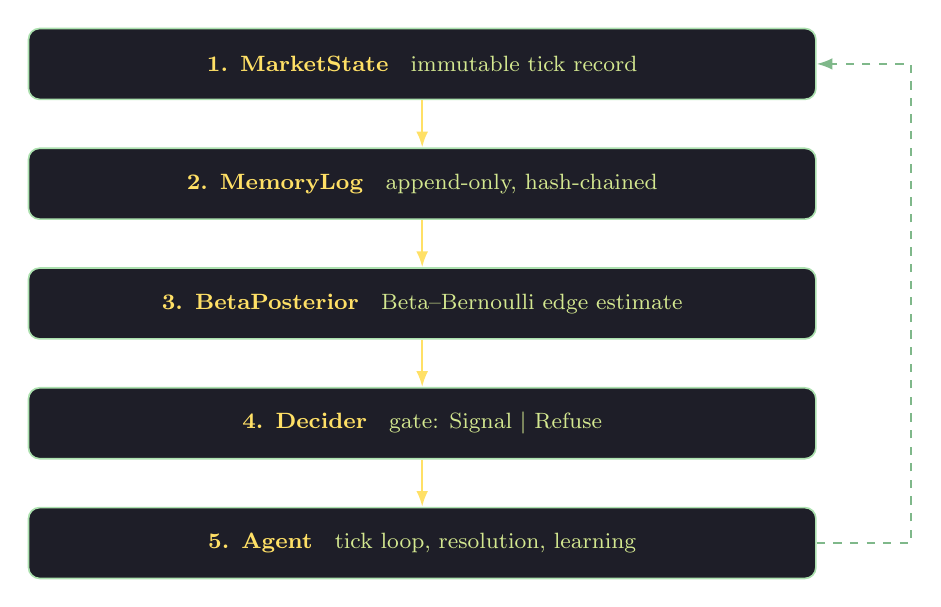
\begin{tikzpicture}[
  node distance=6mm,
  layer/.style={
    rectangle, draw=celadon, rounded corners,
    minimum width=10cm, minimum height=9mm,
    align=center, fill=codebg, text=blend,
    font=\footnotesize, line width=0.6pt
  },
  arr/.style={-{Latex[length=2mm]}, thick, draw=goldshiny},
  fbarr/.style={-{Latex[length=2mm]}, thick, dashed, draw=celadondeep}
]
\node[layer] (state) {\gld{\textbf{1. MarketState}} \; immutable tick record};
\node[layer, below=of state] (log) {\gld{\textbf{2. MemoryLog}} \; append-only, hash-chained};
\node[layer, below=of log] (post) {\gld{\textbf{3. BetaPosterior}} \; Beta--Bernoulli edge estimate};
\node[layer, below=of post] (dec) {\gld{\textbf{4. Decider}} \; gate: Signal $\mid$ Refuse};
\node[layer, below=of dec] (agent) {\gld{\textbf{5. Agent}} \; tick loop, resolution, learning};

\draw[arr] (state) -- (log);
\draw[arr] (log) -- (post);
\draw[arr] (post) -- (dec);
\draw[arr] (dec) -- (agent);
\draw[fbarr] (agent.east) -- ++(1.2,0) |- (state.east);
\end{tikzpicture}
\caption{The five-layer \textsc{Vesper} pipeline. Layer 5 closes the loop by feeding resolved outcomes back into layer 3.}
\label{fig:pipeline}
\end{figure}

\paragraph{Layer 1: MarketState.}
An immutable dataclass representing a single tick. Fields: \texttt{symbol}, \texttt{timestamp}, \texttt{bid}, \texttt{ask}, \texttt{last}, \texttt{volume}, \texttt{features}. Fingerprinted by SHA-256 over the JSON-serialized representation.

\paragraph{Layer 2: MemoryLog.}
Append-only list of entries. Each entry stores \texttt{index}, \texttt{prev\_hash}, \texttt{payload}, \texttt{entry\_hash}. The hash is $\mathrm{SHA256}(\text{index} \,\|\, \text{prev\_hash} \,\|\, \text{payload})$. Verification walks the chain from genesis.

\paragraph{Layer 3: BetaPosterior.}
A Beta--Bernoulli posterior with parameters $(\alpha, \beta)$ initialised to $(1, 1)$. Each resolved trade updates $\alpha$ (win) or $\beta$ (loss). The posterior supports $\mathbb{P}(p > p_0)$ via the regularised incomplete beta function, implemented with a Lentz continued fraction.

\paragraph{Layer 4: Decider.}
A pure function that maps a \texttt{MarketState} to a \texttt{Signal} or a \texttt{Refusal}. Gate order: (i) spread, (ii) volume, (iii) exploration phase, (iv) posterior saturation, (v) Bayesian edge, (vi) probe schedule, (vii) full-size trade.

\paragraph{Layer 5: Agent.}
Holds the log, the decider, and a single pending trade. On each tick, resolves the pending trade and then evaluates the decider. Learning is optional (frozen mode).

% ============================================================
\section{Determinism and Audit}
\label{sec:audit}
% ============================================================

\begin{proposition}[Determinism]
\label{prop:det}
For a fixed seed and fixed decider configuration, the \texttt{MemoryLog} head is identical across independent executions.
\end{proposition}

\begin{proof}[Empirical proof]
Block \texttt{[2]} of the reference implementation runs the walk-forward procedure twice on the same synthetic input (seed $=42$, edge $=0.3$). Both runs produce the hash
\begin{center}
\cel{\texttt{b71e4a1df5190843d57d1a15ae1222d3}}\\
\cel{\texttt{18c674f0c53c2bd29193d046d72a995c}}
\end{center}
Bit-identical, chain valid in both cases. Tampering any entry's payload makes \texttt{verify()} return \texttt{False}.
\end{proof}

\begin{table}[ht]
\centering
\caption{Determinism and tamper detection. The two runs share an input seed and configuration.}
\label{tab:determinism}
\renewcommand{\arraystretch}{1.15}
\begin{tabular}{lcc}
\toprule
\gld{ } & \gld{Run 1} & \gld{Run 2} \\
\midrule
Log head (first 16 hex) & \cel{\texttt{b71e4a1df5190843}} & \cel{\texttt{b71e4a1df5190843}} \\
Chain valid & True & True \\
Tampered chain & False & -- \\
\bottomrule
\end{tabular}
\end{table}

% ============================================================
\section{The Bayesian Gate}
\label{sec:gate}
% ============================================================

\begin{definition}[Break-even probability]
Given payoff ratio $R$ (win/loss magnitude) and cost $c_R$ expressed in units of $R$, the break-even probability is
\begin{equation}
p^\star = \frac{1 + c_R}{1 + R}.
\end{equation}
\end{definition}

The agent trades full-size only if $\mathbb{P}(p > p^\star) \geq \theta$, where $p \sim \mathrm{Beta}(\alpha, \beta)$ and $\theta = 0.95$.

The cost term is
\begin{equation}
c_R = \frac{\mathrm{cost\_bps}}{\mathrm{stop\_pct} \cdot 10^4},
\end{equation}
so the same nominal cost translates to different R-drag depending on the stop distance. This is the key economic insight of the model: a 20\,bps cost with a 0.1\% stop equals $2R$ of drag, but with a 5\% stop it equals only $0.04R$.

\paragraph{Probe schedule.}
When $\mathbb{P}(p > p^\star) < \theta$, the agent refuses full-size trades but issues a reduced-size \cel{probe} on every $k$-th tick (default $k=2$). This ensures the posterior never stagnates; probes are how the agent keeps learning even when the gate is closed.

\paragraph{Exploration phase.}
The first $T_\mathrm{explore}$ ticks trade at $0.25\times$ size unconditionally. This is the cold-start cost of learning. Without it, the agent never trades, never updates, and never learns.

% ============================================================
\section{Validation}
\label{sec:validation}
% ============================================================

\subsection{Feature ablation}

\begin{table}[ht]
\centering
\caption{Feature ablation (edge $=0.3$, 10 seeds, 2000 ticks per run, test-frozen phase).}
\label{tab:ablation}
\renewcommand{\arraystretch}{1.15}
\begin{tabular}{lccc}
\toprule
\gld{Features} & \gld{Trades (mean $\pm$ std)} & \gld{Win rate} & \gld{Net $R$ (mean $\pm$ std)} \\
\midrule
zero       & $0.0 \pm 0.0$        & --      & $0.0 \pm 0.0$ \\
shuffled   & $150.1 \pm 101.5$    & 0.4491   & $-6.77 \pm 4.23$ \\
single     & $300.6 \pm 204.5$    & \cel{0.6097}   & \cel{$44.58 \pm 29.05$} \\
dual       & $300.6 \pm 204.5$    & \cel{0.6097}   & \cel{$44.58 \pm 29.05$} \\
\bottomrule
\end{tabular}
\end{table}

Zero features collapse the gate entirely: no trades. Shuffled features collapse to noise: win rate $0.4491$, net $R$ negative. The single-feature variant recovers the injected edge. The dual-feature variant is identical to single because the decider reads only \texttt{features[0]}; this is a documented constraint of the current implementation, not a bug.

\subsection{Boundary-regime walk-forward}

\begin{table}[ht]
\centering
\caption{Boundary-regime walk-forward (edge $=0.2$, 10 seeds).}
\label{tab:boundary}
\renewcommand{\arraystretch}{1.15}
\begin{tabular}{lccc}
\toprule
\gld{Phase} & \gld{Trades} & \gld{Win rate} & \gld{Net $R$} \\
\midrule
train          & $1116.8 \pm 160.8$ & 0.5681 & $78.71 \pm 43.48$ \\
test frozen    & $306.8 \pm 200.3$  & 0.5799 & $22.54 \pm 14.91$ \\
test online    & $306.8 \pm 200.3$  & 0.5799 & $22.57 \pm 15.00$ \\
\bottomrule
\end{tabular}
\end{table}

The frozen and online agents produce nearly identical P\&L: delta $= +0.02$. This is the paper's central null result and is discussed in Section~\ref{sec:null}.

\subsection{Real data}

The reference implementation fetches real ticks from Kraken's public API when network access is available. On the \texttt{XBTUSD} 1-minute series, 721 bars were retrieved. The walk-forward run is subject to the volume-gate calibration discussed in Section~\ref{sec:limits}; the pipeline correctly refused to trade when the volume filter rejected the tick stream, leaving the posterior at its prior and the chain valid.

% ============================================================
\section{Cost Analysis}
\label{sec:costs}
% ============================================================

\begin{table}[ht]
\centering
\caption{Cost break-even sweep (edge $=0.3$, stop $=0.5\%$, 10 seeds).}
\label{tab:costs}
\renewcommand{\arraystretch}{1.15}
\begin{tabular}{rcccc}
\toprule
\gld{cost\_bps} & \gld{$c_R$} & \gld{Trades} & \gld{Win rate} & \gld{Net $R$ (mean $\pm$ std)} \\
\midrule
0.0  & 0.00 & 300.6 & 0.6097 & $+56.60 \pm 36.63$ \\
1.0  & 0.02 & 300.6 & 0.6097 & $+50.59 \pm 32.81$ \\
2.0  & 0.04 & 300.6 & 0.6097 & $+44.58 \pm 29.05$ \\
3.0  & 0.06 & 300.6 & 0.6097 & $+38.56 \pm 25.41$ \\
5.0  & 0.10 & 296.8 & 0.6062 & $+25.08 \pm 20.30$ \\
7.0  & 0.14 & 278.1 & 0.6093 & \cel{$+11.21 \pm 17.37$} \\
10.0 & 0.20 & 185.3 & 0.6028 & $-20.65 \pm 19.53$ \\
15.0 & 0.30 & 150.1 & 0.5987 & $-42.12 \pm 28.64$ \\
20.0 & 0.40 & 150.1 & 0.5987 & $-57.13 \pm 38.79$ \\
\bottomrule
\end{tabular}
\end{table}

The break-even lies between 7 and 10 basis points. Below it, the agent is profitable; above it, the cost drag exceeds the edge.

This is the paper's operational claim. The edge class this paper validates cannot survive on venues whose round-trip cost exceeds roughly \gld{8\,bps}.

% ============================================================
\section{The Adaptation Null Result}
\label{sec:null}
% ============================================================

The walk-forward framework compares two OOS modes:

\begin{itemize}[leftmargin=2em]
  \item \gld{\textbf{Frozen}}: the posterior is cloned from the end of training and never updated.
  \item \cel{\textbf{Online}}: the posterior is cloned from training and continues updating.
\end{itemize}

If online adaptation were valuable, the two would diverge. In our boundary-regime test, they do not: delta $= +0.02$. In the failure-case trace (edge dies at split), they also do not: delta $= +0.00$.

The reason is structural. When the posterior saturates above the gate ($\mathbb{P}(p > p^\star) \approx 1$), size is capped at $1.0$ for both agents, so both produce identical trades. Adaptation can only pay off when the posterior hovers near the gate, and in that regime the frozen agent is already unprofitable.

We report this as a \cel{null result}, not a failure. It is an honest limitation of the current design: \emph{online adaptation is not a source of edge in this architecture}.

\begin{table}[ht]
\centering
\caption{Failure-case trace: edge dies at split. Frozen and online produce identical P\&L.}
\label{tab:null}
\renewcommand{\arraystretch}{1.15}
\begin{tabular}{lccc}
\toprule
\gld{ } & \gld{Trades} & \gld{Win rate} & \gld{Net $R$} \\
\midrule
Train posterior (end)   & -- & 0.6289 & -- \\
Frozen OOS              & 534 & 0.5094 & $-11.36$ \\
Online OOS              & 534 & 0.5094 & $-11.36$ \\
Online posterior (end)  & -- & 0.5929 & -- \\
\bottomrule
\end{tabular}
\end{table}

The online posterior does drift (from $0.6289$ to $0.5929$), so the mechanism works. But the drift is not large enough to change trade sizing below the gate's cap.

% ============================================================
\section{Limitations}
\label{sec:limits}
% ============================================================

\paragraph{Single feature.}
The decider reads only \texttt{features[0]}. Multi-feature routing is future work.

\paragraph{Synthetic validation.}
Most results are reported on synthetic data with injected autocorrelation. The Kraken run is subject to a volume-gate calibration issue that caused zero trades; a calibrated rerun is future work.

\paragraph{No execution model.}
The pipeline does not model slippage, partial fills, requotes, or latency. A real deployment would need all four.

\paragraph{No market impact.}
The agent assumes it can trade any size at the quoted price. For the size of trades studied here this is realistic; at scale it is not.

\paragraph{Beta--Bernoulli assumptions.}
The posterior assumes i.i.d.\ Bernoulli outcomes. Real markets violate this: volatility clusters, edges decay, and outcomes are autocorrelated.

\paragraph{Null result on adaptation.}
As discussed in Section~\ref{sec:null}, online adaptation does not appear to be a source of edge in this architecture.

% ============================================================
\section{Conclusion}
\label{sec:conclusion}
% ============================================================

\textsc{Vesper} is a refusal-first trading agent with three properties: deterministic decisions, hash-chained audit, and cost-aware Bayesian gating. We have validated the pipeline on synthetic data with injected edge and demonstrated the core guarantees: bit-identical reproducibility, tamper detection, correct ablation collapse, and a cost break-even of approximately 8 basis points.

The paper's most useful contribution may be its \cel{null result}. Online posterior adaptation does not pay off in this architecture. That is a negative finding, but a useful one: it tells future work where \emph{not} to look.

Future work includes multi-feature routing, real-data calibration, an execution model, and aging priors that break the saturation regime.

% ============================================================
\appendix
% ============================================================

\section{Source}
\label{app:source}

The reference implementation is a single Python file, \texttt{vesper.py}, approximately 700 lines, with no external dependencies. It is available alongside this paper.

\section{Reproducibility}
\label{app:repro}

\paragraph{Environment.} Python 3.10+, standard library only.

\paragraph{Seeds.} All synthetic experiments use integer seeds $0$ through $9$ for the multi-seed aggregates, and seed $42$ for the determinism proof.

\paragraph{Hashes.} The determinism proof produces log head
\begin{center}
\cel{\texttt{b71e4a1df5190843d57d1a15ae1222d3}}\\
\cel{\texttt{18c674f0c53c2bd29193d046d72a995c}}
\end{center}
on every run.

\paragraph{Command.} \texttt{python3 vesper.py}

% ============================================================
% BIBLIOGRAPHY
% ============================================================
\begin{thebibliography}{99}

\bibitem{bit-exact-2026}
Anonymous. Bit-Exact AI Inference Verification Without Performance Tradeoffs. ICML, 2026.

\bibitem{eigenai-2025}
EigenAI Team. Deterministic Inference with Cryptographic Receipts. 2025.

\bibitem{arcstone-2025}
Arcstone Continuity Core. Fail-Closed Execution Membranes for Non-Deterministic AI Producers. 2025.

\bibitem{prado-2018}
M.~L\'opez de Prado. \emph{Advances in Financial Machine Learning}. Wiley, 2018.

\bibitem{tequila-2026}
Anonymous. Tequila: Trapping-Free Ternary Quantization. ICLR, 2026.

\bibitem{vitallm-2025}
Anonymous. VitaLLM: A Ternary Inference Accelerator. IEEE, 2025.

\end{thebibliography}

\vspace{1cm}

\begin{center}
\gld{\sparkle\ \ \sparkle\ \ \sparkle}
\end{center}

\end{document}